\chapter{Тарифный принцип, нагрузка в явном и неявном виде. Порядок отношения правдоподобия и экспоненциальный порядок.}
\problem{}
Пусть число наступления событий $N$ имеет распределение Пуассона с параметром $\lambda$. События классифицируются на $m$ групп, причем каждое из них, независимо от остальных, принадлежит $i$-й группе с вероятностью $p_i$. Тогда случайные величины $N_i$, $i =\overline{1,m}$, независимые пуассоновские с параметрами $p_i\lambda$. ($N_i$ - число событий в группе $i$.)

\solution{}
    Пусть $\eta_k$ -- номер класса события $k$. Тогда
    \begin{equation}
        \P(\eta_k = i) = p_i.
    \end{equation}
    Из условия задачи имеем
    \begin{equation}
        N_i = \sum_{k:\ \eta_k = i} 1 = \sum_k \1(\eta_k = i).
    \end{equation}
    Найдем искомое распределение:
    \begin{multline}
        \P(N_i = n) =
        \sum_{k=0}^\infty \P\left(N=k, \sum_{n=1}^k\1(\eta_k = i) = n\right) =\\=
        \sum_{k=n}^\infty \P\left(N=k, \sum_{n=1}^k\1(\eta_k = i) = n\right) =\\=
        \sum_{k=n}^\infty \P\left(N=k\right) \P\left(\sum_{n=1}^k\1(\eta_k = i) = n\right) =\\=
        \sum_{k=n}^\infty \frac{\lambda^k}{k!}e^{-\lambda} \binom{k}{n}p_i^n(1-p_i)^{k-n} =\\=
        \sum_{k=n}^\infty e^{-\lambda} \frac{\lambda^k}{k!}\frac{k!}{n!(k-n)!} p_i^n(1-p_i)^{k-n} =\\=
        \sum_{k=n}^\infty e^{-\lambda} \frac{\lambda^k}{n!(k-n)!} p_i^n(1-p_i)^{k-n} =\\=
        \frac{p_i^ne^{\lambda}\lambda^n}{n!}\sum_{k=0}^\infty\frac{(\lambda(1-p_i))^{k}}{k!}  =
        \frac{(\lambda p_i)^n}{n!}e^{-\lambda p_i}.
    \end{multline}
    Получили искомое распределение. Остается проверить независимость. Это свойство очевидно следует из независимости $\eta_k$.

\problem{}
Проверить, что биномиальные распределения с параметрами $n$ и $p$ растут стохастически по $p$ при фиксированном $n$ и стохастически растут по $n$ при фиксированном $p$.

\solution{}
    1. Фиксируем $n$. Пусть $p_1 < p_2$. Тогда хотим
        \begin{equation}
            \P(X_1 = k) = \binom{n}{k}p_1^k(1-p_1)^{n-k} \geq \binom{n}{k}p_2^k(1-p_2)^{n-k} = P(X_2 = k).
        \end{equation}
        На биномиальный коэффициент можно не обращать внимания, так как он не зависит от $p$. Тогда нужно проверить неравенство
        \begin{equation}
            p_1^k(1-p_1)^{n-k} \geq p_2^k(1-p_2)^{n-k}.
        \end{equation}
        Обозначим $a = p_2/p_1 > 1, p_1 = p$. Имеем:
        \begin{equation}\label{to1}
             \underbrace{a^k}_{<1} \left(\frac{1-ap}{1-p}\right)^{n-k} <...?
        \end{equation}
        \begin{equation}
            \frac{1-ap}{1-p}\ \ ?\ \ 1
        \end{equation}
        \begin{equation}
            1-ap\ \ ?\ \ 1-p
        \end{equation}

        Отсюда следует, что $?$ это $<$. 
        Таким образом, в \eqref{to1} можно поставить $1$ вместо многоточия, и имеем стохастическую монотонность.

    2. Фиксируем $p$. Пусть $n_1 < n_2$. Тогда хотим
        \begin{equation}
            \P(X_1 = k) = \binom{n_1}{k}p^k(1-p)^{n_1-k} \geq \binom{n_2}{k}p^k(1-p)^{n_2-k} = P(X_2 = k).
        \end{equation}
        Хотим \begin{equation}
            \frac{n_1!}{(n_1 - k)!}(1-p)^{n_1} \geq \frac{n_2!}{(n_2 - k)!}(1-p)^{n_2}
        \end{equation}
        Хотим \begin{equation}
            \frac{n_1!}{n_2!}\frac{(n_2 - k)!}{(n_1 - k)!}(1-p)^{n_1-n_2} \geq 1
        \end{equation}
        Имеем
        \begin{equation}
            \frac{n_1!}{n_2!}\frac{(n_2 - k)!}{(n_1 - k)!}(1-p)^{n_1-n_2} \geq \frac{n_1!}{n_2!}\frac{(n_2 - n_1)!}{1}(1-p)^{n_1-n_2} > 1
        \end{equation}

\problem{}
Верно ли, что $D Y \geq D X$, если $X <_v Y$?

\solution{}
    Пусть $X <_v Y$. По определению это означает, что $\exists Z\colon \E\left[Z|X\right] \overset{\text{a.s.}}{\geq} 0$ и $X+Z \overset{\text{law}}{=} Y$.
    Более того, знаем, что $X<_vY \iff X<_{sl}Y, X<_{st}Y$. А отсюда следует необходимость данного стохастического порядка.
    Рассмотрим\begin{enumerate}
        \item $X \sim U[1, 3]$, $\var X = 1/3$;
        \item $Y\sim U[3, 4]$, $\var Y = 1/12$.
    \end{enumerate}
    Есть стохастический и стоп-лосс, а значит, выполнено $X<_vY$. Но $\var X > \var Y$, что противоречит условию.

\problem{}
Пусть риск $X$ равномерно распределен на $[0, 2]$, а $Y$ имеет показательное распределение с параметром 1, тогда $X <_{sl} Y$ .

\solution{}
    Пусть $0 < d < 2$. 
    \begin{align}
        \E\left[(X - d)^+\right] &= 0.5 \int_{d}^{2} (x-d) dx = 0.5 \frac{4 - d^2}{2} + 0.5(d-2)d = 1 - d + 0.25d^2, \\
        \E\left[(Y - d)^+\right] &= \int_{d}^{\infty} (y-d) e^{-(y-d) - d} dy = e^{-d} \int_{0}^{\infty} y e^{-y} dy = e^{-d}.
    \end{align}
    \begin{figure}[htbp]
        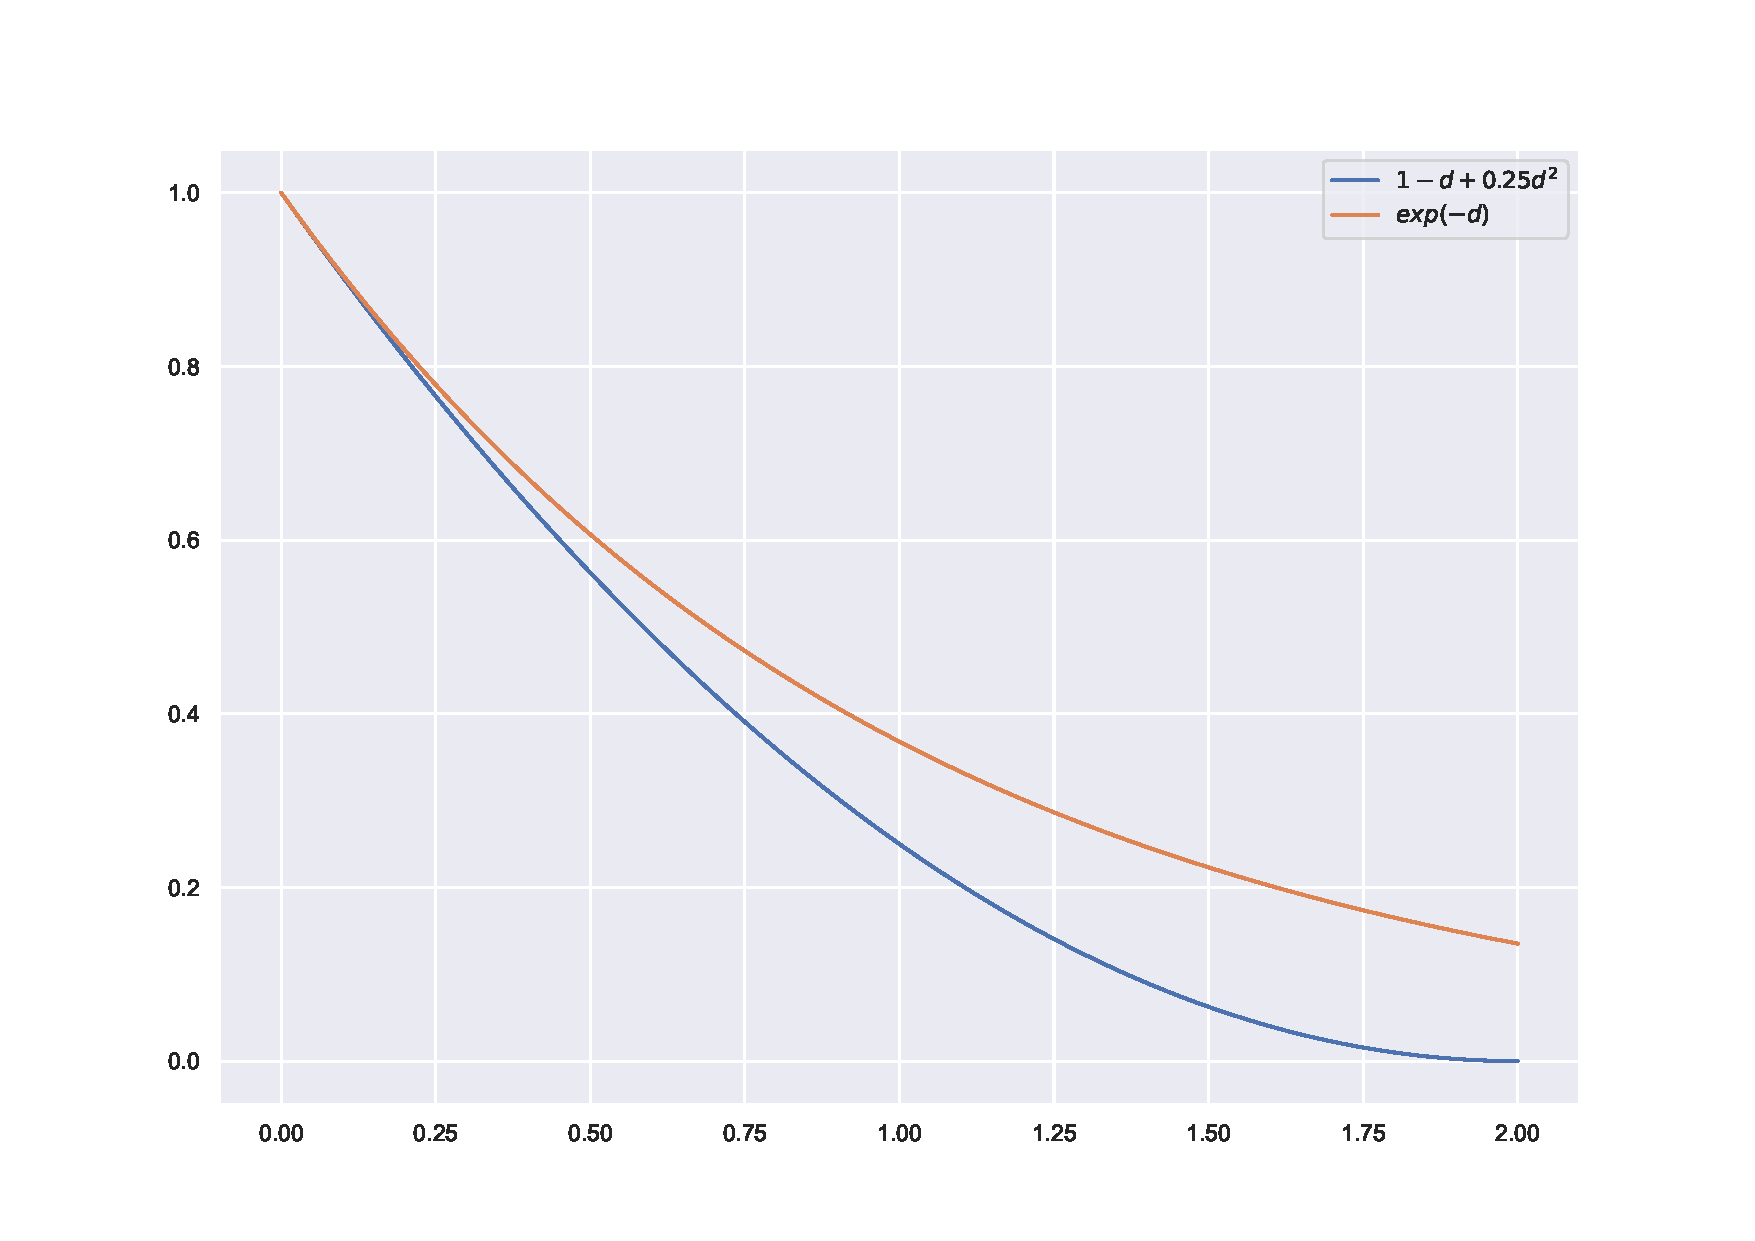
\includegraphics[width=\textwidth]{pics/hw6t4p1.pdf}
        \caption{Графики функций $\E\left[(X - d)^+\right]$ и $\E\left[(Y - d)^+\right]$ при $d\in[0, 2]$}
    \end{figure}
    Очевидно, что когда $d \geq 2$, то $0 = \E\left[(X - d)^+\right] < \E\left[(Y - d)^+\right]$. Таким образом, $X <_{sl} Y$.